%Cap�tulo 2: Ingenir�a de Requerimientos

\chapter{Ingenier�a de Requerimientos}

\section{Introducci�n}

\subsection{Definici�n}

Todo Software se desarrolla con un \emph{prop�sito}. Luego podemos definir \emph{calidad} como el grado con que el software cumple con el prop�sito.

La \emph{\textbf{Ingenier�a de Requerimientos (RE)}} es un conjunto de actividades concernientes a identificar y comunicar el prop�sito de un sistema intensivo de software y el contexto en que ser� usado. 

Tanto el problema como la soluci�n son el resultado del comportamiento emergente de la interacci�n entre los componentes del sistema. Por eso hablamos de Ingenier�a de Requerimientos de \emph{Sistemas Intensivos en Software} (Software + Hardware + Entorno).

Por lo tanto la Ingenier�a de Requerimientos act�a como puente entre las necesidades del mundo real de los usuarios, clientes y otros individuos afectados por el sistema de software, y las capacidades y oportunidades surgidas a partir de las tecnolog�as de software intensivo.

\subsection{Separaci�n del problema y la soluci�n}

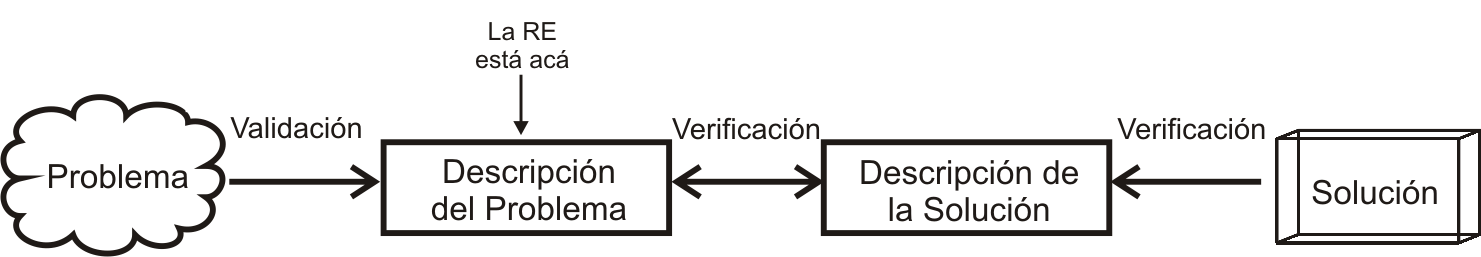
\includegraphics[width = 0.9\textwidth]{Graficos/separacion.png}

La Ingenier�a de Requerimientos requiere controlar que:

\begin{itemize}
	\item El problema se corresponde con lar verdaderas necesidades (validaci�n)
	\item La soluci�n correctamente resuelve la descripci�n del problema (verificaci�n)
\end{itemize}

\subsection{Actividades de Ingenier�a de Requerimientos}

\begin{description}
	\item[Elicitaci�n:] evocar una respuesta de alguien como reacci�n a preguntas o acciones.
	\item[Modelado:] documentar rigurosamente para an�lisis (abstraer y estructurar lo elicitado)
	\item[An�lisis:] verificaci�n inter e intra modelos
	\item[Validaci�n:] �los modelos se corresponden con la realidad?
	\item[Priorizaci�n:] establecer criterios de preferencia con respecto a alcance y objetivos.
	\item[Negociaci�n:] unificar criterios entre los interesados
	\item[Especificaci�n:] documentaci�n completa y detallada (documento final) 
\end{description}

\section{Modelo de Jackson}
\comentario{completar}

\section{Modelo de las 4 variables}
\comentario{completar}

\section{Diagrama de Contexto}
\comentario{completar}

\section{Modelo de Objetivos}
\comentario{completar}

\section{Modelo de Operaciones}
\comentario{completar}

\section{Modelo Conceptual}
\comentario{completar}

\section{Modelos de Comportamiento}
\comentario{completar}
